\iffalse
\documentclass[12pt]{article}
\usepackage{graphicx}
%\documentclass[journal,12pt,twocolumn]{IEEEtran}
\usepackage[none]{hyphenat}
\usepackage{graphicx}
\usepackage{gensymb}
\usepackage{listings}
\usepackage[english]{babel}
\usepackage{graphicx}
\usepackage{caption}
\usepackage[parfill]{parskip}
\usepackage{hyperref}
\usepackage{booktabs}
%\usepackage{setspace}\doublespacing\pagestyle{plain}
\def\inputGnumericTable{}
\usepackage{color}                                            %%
    \usepackage{array}                                            %%
    \usepackage{longtable}                                        %%
    \usepackage{calc}                                             %%
    \usepackage{multirow}                                         %%
    \usepackage{hhline}                                           %%
    \usepackage{ifthen}
\usepackage{array}
\usepackage{amsmath}   % for having text in math mode
\usepackage{parallel,enumitem}
\usepackage{listings}
\lstset{
language=tex,
frame=single,
breaklines=true
}
 
%Following 2 lines were added to remove the blank page at the beginning
\usepackage{atbegshi}% http://ctan.org/pkg/atbegshi
\AtBeginDocument{\AtBeginShipoutNext{\AtBeginShipoutDiscard}}
%
%New macro definitions
\newcommand{\mydet}[1]{\ensuremath{\begin{vmatrix}#1\end{vmatrix}}}
\providecommand{\brak}[1]{\ensuremath{\left(#1\right)}}
\providecommand{\norm}[1]{\left\lVert#1\right\rVert}
\newcommand{\solution}{\noindent \textbf{Solution: }}
\newcommand{\myvec}[1]{\ensuremath{\begin{pmatrix}#1\end{pmatrix}}}
\let\vec\mathbf
\begin{document}
\begin{center}
\enlargethispage{-4cm}
\title{\textbf{Three Dimensional Geometry}}
\date{\vspace{-5ex}} %Not to print date automatically
\maketitle
\end{center}
\setcounter{page}{1}
\section*{12$^{th}$ Maths - Chapter 11}
This is Problem-3 from Exercise 11.1
\begin{enumerate}

\solution
\fi
The input parameters are available in Table \ref{tab:chapters/10/10/1/3/}.
\begin{table}[H]\centering
\begin{tabular}{|p{3cm}|p{3cm}|p{3cm}|}
\hline                                        
\textbf{Symbol} & \textbf{Values} & \textbf{Description}\\                                          
\hline                                 
$\theta$ & 30$\degree{}$   & $\angle{BAD} = \angle{BAC}$ \\           
\hline                                    
a &  9 & $AB$ \\     
\hline                      
c & 5 & $AC$ \\
\hline                                     
		$\vec{e}_1$ & $\myvec{
			1\\
			0\\
			}$ & basis vector\\ 
\hline
\end{tabular}

\caption{}
\label{tab:chapters/10/10/1/3/} 
\end{table}
From the given information, 	
\begin{align}
	\norm{\vec{Q}}^2&=d^2\label{eq:chapters/10/10/1/3/1}
	\\
\brak{\vec{Q}-\vec{P}}^{\top}\vec{P}&=0 \implies
\vec{P}^{\top}\vec{Q}=\norm{\vec{P}}^2=r^2\\
	\text{or, }	\vec{P}^{\top}\vec{Q}&=25\label{eq:chapters/10/10/1/3/4}
\end{align}
For $\theta=0\degree$ 
\begin{align}
\vec{P}=\myvec{5\\0}
\end{align}
Substituting the above in \eqref{eq:chapters/10/10/1/3/4},
\begin{align}
\myvec{5&0}\vec{Q}&=25\\
\implies 
	\vec{Q}&=\myvec{5\\0}+\mu\myvec{0\\1}\label{eq:chapters/10/10/1/3/9}
\end{align}
	which is of the form 
\begin{align}
	\vec{Q}=\vec{A}+\mu\vec{m}\label{eq:chapters/10/10/1/3/10}
\end{align}
		Then substituting \eqref{eq:chapters/10/10/1/3/10} in \eqref{eq:chapters/10/10/1/3/1} yeilds,
\begin{align}
	&\implies\brak{\vec{A}+\mu\vec{m}}^{\top}\brak{\vec{A}+\mu\vec{m}}=d^2\\
	&\implies \mu^2\norm{\vec{m}}^2+2\mu\vec{A}^{\top}\vec{m}+\norm{\vec{A}}^2=d^2\label{eq:chapters/10/10/1/3/14}
\end{align}
where
\begin{align}
	\vec{A}=\myvec{5\\0}\text{ and }\vec{m}=\myvec{0\\1}
\end{align}
	Substituting numerical values, 
\begin{align}
\mu^2=119
	\implies\mu=\pm\sqrt{119}
\end{align}
yeilding 
\begin{align}
\vec{Q_1}=\myvec{5\\\sqrt{119}},\vec{Q_2}=\myvec{5\\-\sqrt{119}}
\end{align}
Thus, 
\begin{align}
	PQ_1 = PQ_2  = \sqrt{119}
\end{align}
See Fig. 
\ref{fig:chapters/10/10/1/3/Fig1}.
\begin{figure}[H]
\begin{center}
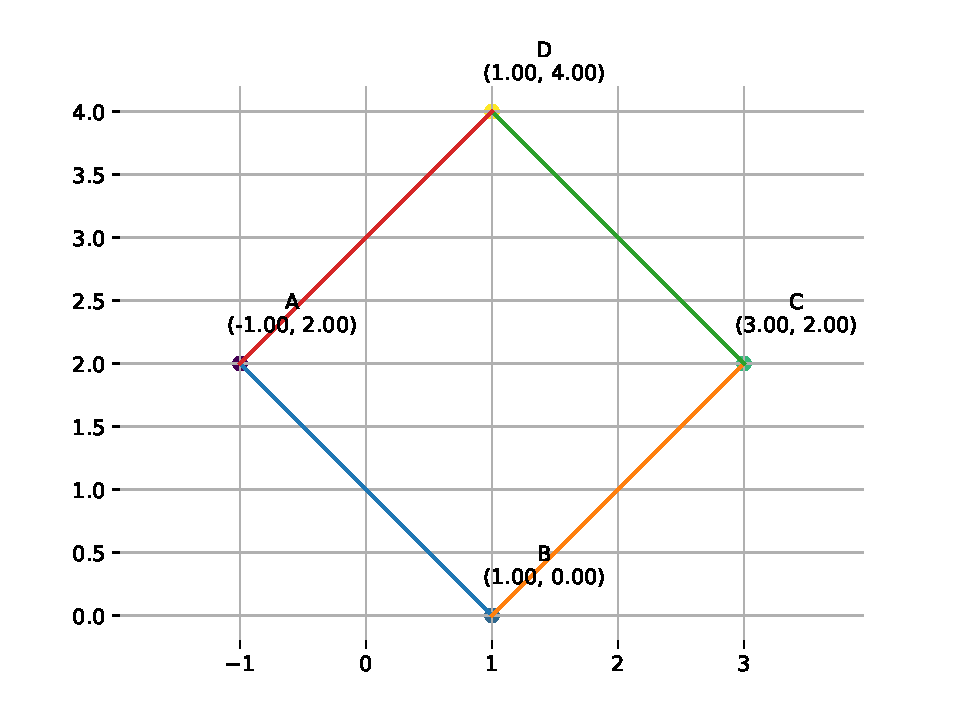
\includegraphics[width=0.75\columnwidth]{chapters/10/10/1/3/figs/fig2.pdf}
\end{center}
\caption{}
\label{fig:chapters/10/10/1/3/Fig1}
\end{figure}
